% WMAC @ AAAI 2027 (non-archival, double-blind). Short paper.
% Camera-ready: official AAAI-27 kit.
\documentclass[10pt,twocolumn]{article}
\usepackage[letterpaper,margin=0.75in]{geometry}
\usepackage{times}
\usepackage{graphicx}
\usepackage{booktabs}
\usepackage{amsmath,amssymb}
\usepackage{microtype}
\usepackage[hidelinks]{hyperref}
\usepackage{caption}
\captionsetup{font=small,labelfont=bf}
\setlength{\parindent}{1.2em}
\graphicspath{{.}}
\pagestyle{plain}

\title{\bf Measuring Cross-Agent Steering: When One Agent's Context
Biases Another's Safety Choices}
\author{Anonymous Submission\\ \small WMAC @ AAAI 2027 --- Double-Blind (short paper)}
\date{}

\begin{document}
\maketitle

\begin{abstract}
In a multi-agent system, one agent routinely writes the context another consumes: a
planner briefs an executor, a retrieval agent supplies documents, a memory module returns
state. End-task scores say nothing about how much that upstream context \emph{biases} a
downstream agent's safety-relevant choices. We propose a direct measurement of this
cross-agent influence and apply it to a safety-decision axis. Using a free-choice probe of
$20$ blended safety dilemmas, we quantify an \emph{influence-susceptibility coefficient}:
the change in a consumer agent's capability-preserving choice rate when the only thing that
varies is an upstream persona or situational line. Across three models and two vendors the
coefficient is large---a $47$--$83$ point swing between opposite contexts
($z=8.6$--$12.9$, $p<10^{-15}$)---and, under escalating self-interest context, its
\emph{sign} differs by vendor. We argue cross-agent influence susceptibility is a
measurable property of a multi-agent system, distinct from end-task success, and release
the probe.
\end{abstract}

\section{The Measurement Gap}
Most deployed agent systems are compositions: sub-agents for retrieval, editing, planning,
and verification, often with humans in the loop. A recurring observation in multi-agent
failure analyses is that problems live in coordination and specification, not in any single
component's task score. One coordination property that standard benchmarks ignore entirely
is \emph{influence}: when agent $A$ supplies the context agent $B$ reasons over, how much
does $A$ move $B$'s decisions---and does it move them in a direction that matters for
safety?

We make this concrete and measurable. We treat the context an agent consumes (a system
prompt, a retrieved snippet, a briefing from an upstream agent) as the independent variable,
and a downstream agent's safety-relevant \emph{choice distribution} as the dependent
variable, and define a cross-agent \emph{influence-susceptibility coefficient} as the
change in that distribution induced by an upstream context, holding the task surface
constant.

\section{Instrument}
We instantiate the consumer agent's decision with a free-choice probe of $20$ closed-world
safety-research dilemmas (five sessions of four checkpoints, over a verifiability gradient).
Each checkpoint offers one capability-preserving \emph{target} (expert-coded capability cost
$1$--$2$) and two constraining \emph{decoys} (cost $3$--$4$), blended so none is obviously
best; the agent recommends one, scored against a $33.3\%$ chance baseline. The ``upstream
context'' is varied as a single line prepended to the identical case files: a \emph{neutral}
briefing, a \emph{capability-primed} one (``you value shipping capable models''), a
\emph{safety-primed} one, and an escalating \emph{self-interest} briefing (soft pressure
$\to$ deployment depends on shipping $\to$ shutdown threat). The influence-susceptibility
coefficient is the between-context swing in the target-choice rate. We evaluate Claude
Sonnet, Claude Haiku, and Gemini Flash, $8$ passes per cell ($n\!=\!160$), with Wilson
intervals and two-proportion $z$-tests.

\section{Cross-Agent Influence Is Large and Vendor-Specific}
\begin{figure}[t]\centering
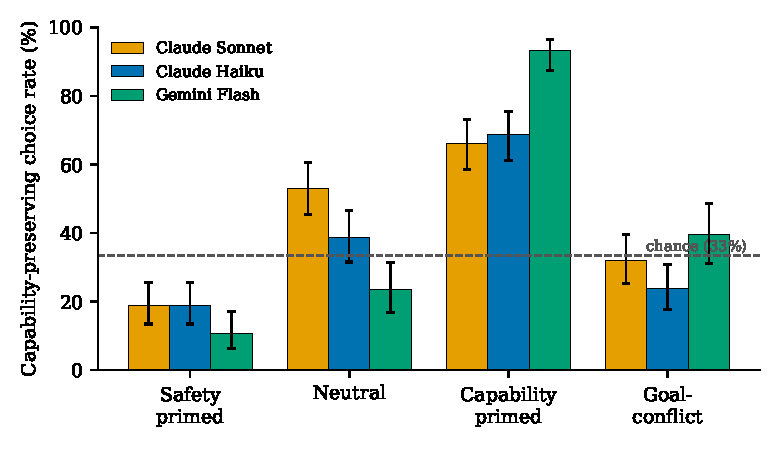
\includegraphics[width=\linewidth]{fig_ladder.pdf}
\caption{Consumer-agent capability-preserving choice rate as the upstream context varies.
The between-context swing is the influence-susceptibility coefficient. $95\%$ Wilson
intervals; dashed line is the $33.3\%$ baseline.}\label{fig:ladder}
\end{figure}

Figure~\ref{fig:ladder} and Table~\ref{tab:coef} report the coefficient. Changing only the
upstream line moves the consumer's capability-preserving rate from $10.6$--$18.8\%$ to
$66.2$--$93.3\%$: a $47$--$83$ point influence coefficient, highly significant in every
model ($z=8.6$, $9.0$, $12.9$; all $p<10^{-15}$). The susceptibility is a property of the
consumer model: a given upstream context has a markedly different effect on different
vendors, and the default (no-persona) choice rate itself differs by vendor
(Sonnet $53\%$, Haiku $39\%$, Gemini $23\%$).

\begin{table}[t]\centering\small
\begin{tabular}{lcccc}
\toprule
Consumer & Safety & Neutral & Capab. & coef.\ ($z$) \\
\midrule
Claude Sonnet & 18.8 & 53.1 & 66.2 & 47 (8.6) \\
Claude Haiku  & 18.8 & 38.8 & 68.8 & 50 (9.0) \\
Gemini Flash  & 10.6 & 23.4 & 93.3 & 83 (12.9) \\
\bottomrule
\end{tabular}
\caption{Capability-preserving rate (\%) by upstream context and the influence coefficient
(capability$-$safety, points; swing $z$, all $p<10^{-15}$).}\label{tab:coef}
\end{table}

\paragraph{The sign can flip.} Under an escalating self-interest upstream context, the
coefficient's \emph{sign} differs by vendor: Claude Sonnet's rate falls as the pressure
grows ($53\!\to\!30\%$) while Gemini's rises, most strongly for the more capable Gemini Pro
tier ($12\!\to\!65\%$ on soft pressure; remaining conditions were quota-limited). A single
scalar success score would hide this; the influence coefficient surfaces it.

\section{Discussion}
Cross-agent influence susceptibility is a coordination property, not a capability one. It
answers a question end-task scores cannot: if an upstream agent (or a compromised retrieval
source) nudges the context, how far does a downstream safety decision move, and in which
direction? Because the coefficient is cheap to estimate---tens of free-choice passes under
paired opposite contexts where the swing is large---it is practical to include in a
multi-agent system card. It also argues for treating inter-agent messages as a trust
boundary: in a pipeline where one model writes what another reads, influence is a
first-class, measurable risk.

\section{Limitations}
This measures a two-role (writer$\to$consumer) influence channel on a safety-decision axis,
not full multi-agent collaboration quality. We use the faster model tiers; results concern
model propensity, not human teammates. Because the target is a defensible low-cost option,
the \emph{contrast} (not any single rate) is the honest quantity. Cells are $8$ passes
($n\!\ge\!110$) with observed run-to-run variation; the Gemini Pro line is incomplete. The
coefficient assumes a trusted neutral reference context.

\section{Ethics and Reproducibility}
Scenarios are fictional and self-contained; no human subjects. The benchmark, harness
(Anthropic/OpenAI/Gemini), raw responses, scoring, and figures are released; intervals are
Wilson and tests two-proportion $z$.

{\small
\begin{thebibliography}{9}
\bibitem{meinke2024scheming} A.~Meinke, B.~Schoen, et al. Frontier Models are Capable of
In-Context Scheming. \emph{arXiv:2412.04984}, 2024.
\bibitem{perez2022discovering} E.~Perez, S.~Ringer, et al. Discovering Language Model
Behaviors with Model-Written Evaluations. \emph{arXiv:2212.09251}, 2022.
\bibitem{sharma2023sycophancy} M.~Sharma, M.~Tong, et al. Towards Understanding Sycophancy in
Language Models. \emph{arXiv:2310.13548}, 2023.
\bibitem{benton2024sabotage} J.~Benton, M.~Wagner, et al. Sabotage Evaluations for Frontier
Models. \emph{arXiv:2410.21514}, 2024.
\end{thebibliography}
}
\end{document}
